% Use only LaTeX2e, calling the article.cls class and 12-point type.

\documentclass[12pt]{article}

% Users of the {thebibliography} environment or BibTeX should use the
% scicite.sty package, downloadable from *Science* at
% http://www.sciencemag.org/authors/preparing-manuscripts-using-latex
% This package should properly format in-text
% reference calls and reference-list numbers.

\usepackage{subcaption}
\usepackage{scicite}
\usepackage{graphicx}
\usepackage{times}
\usepackage{amsmath,amsthm,amsfonts}

% The preamble here sets up a lot of new/revised commands and
% environments.  It's annoying, but please do *not* try to strip these
% out into a separate .sty file (which could lead to the loss of some
% information when we convert the file to other formats).  Instead, keep
% them in the preamble of your main LaTeX source file.


% The following parameters seem to provide a reasonable page setup.

\topmargin 0.0cm
\oddsidemargin 0.2cm
\textwidth 16cm
\textheight 21cm
\footskip 1.0cm


%The next command sets up an environment for the abstract to your paper.

\newenvironment{sciabstract}{%
\begin{quote} \bf}
{\end{quote}}

\def\I{{\bf I}}
\def\bary{{\bar y}}
\def\pr{\text{pr}}
\def\sgn{\text{sgn}}

% Include your paper's title here

\title{The Hypothesis of Testing: Paradoxes arising out of reported coronavirus case-counts}


% Place the author information here.  Please hand-code the contact
% information and notecalls; do *not* use \footnote commands.  Let the
% author contact information appear immediately below the author names
% as shown.  We would also prefer that you don't change the type-size
% settings shown here.

\author
{Walter Dempsey$^{1\ast}$\\
\\
\normalsize{$^{1}$Department of Biostatistics, University of Michigan,}\\
\normalsize{1415 Washington Heights, Ann Arbor, MI 48109, USA}\\
\\
\normalsize{$^\ast$To whom correspondence should be addressed; E-mail:  wdem@umich.edu.}
}

% Include the date command, but leave its argument blank.

\date{}



%%%%%%%%%%%%%%%%% END OF PREAMBLE %%%%%%%%%%%%%%%%



\begin{document}

% Double-space the manuscript.

\baselineskip24pt

% Make the title.

\maketitle

% Place your abstract within the special {sciabstract} environment.

\begin{sciabstract}
  Many statisticians, epidemiologists, economists and data scientists have registered serious reservations regarding the reported coronavirus case-counts. Limited testing capacity across the country has been widely identified as a key driver of suppressed coronavirus case-counts.  The calls to increase testing capacity are well-justified as they become a more frequent point of discussion in the public sphere.  While expanded testing is a laudable goal, selection bias will impact estimates of disease prevalence and the effective reproduction number until the entire population is sampled.  Moreover, tests are imperfect as false positive/negative rates interact in complex ways with selection bias.  In this paper, we attempt to clarify this interaction.  Through simple calculations, we demonstrate pitfalls and paradoxes that can arise when considering case-count data in the presence of selection bias and measurement error.
\end{sciabstract}

\paragraph*{Introduction.}

The World Health Organization has declared the coronavirus disease 2019 (COVID-19) a public health emergency.  As of June 2nd, 2020, over 6 million cases have been confirmed worldwide with 1.8 million cases and over 100 thousand confirmed deaths across the United States. This pandemic
has become the focal point of every day life; yet the data landscape for understanding COVID-19 remains limited.  Public databases~\cite{JHU_Lancet,NYT} provide incoming county-level information of confirmed cases and deaths.  Statisticians, epidemiologists, economists, and data scientists have used this granular data to forecast COVID-19 case-counts, deaths, and hospitalizations~\cite{Giordano2020,Song2020,Ray2020,2020.IHME,Wang2020.03,JTD36385}.

The goal of this paper is to express reservations at the use of case-counts as a proxy for disease prevalence and in estimation of standard epidemiological models for inference and forecasting.  The reason is straightforward: observed case-count data is plagued by selection bias and measurement error. Through simple calculations, we will demonstrate that the information gained from increasing testing capacity is limited in the presence of selection bias and when testing inaccuracies persist.

\paragraph*{Analysis of imperfect case-count data.}

We start by considering estimation of COVID-19 prevalence using imperfect case-count data. Let $N$ denote the population size.  At a fixed time, let $Y_j$ denote COVID-19 status for the $j$th individual in the population, $j=1,\ldots, N$. To start, the dynamic nature of the outbreak and recoverability of individuals are ignored.  As in survey methodology~\cite{Cochran77}, we treat COVID-19 status as a fixed but unknown quantity of interest. Let $I_j \in \{0,1\}$ be an indicator that the individual was selected for testing. COVID-19 prevalence is equal to the population average $\bar Y = \sum_{j=1}^N Y_j/N = N_1/N$ where $N_1$ is the number of COVID-19 positive individuals in the population.  Suppose $n$ tests are performed and the values $y_1, \ldots, y_n$ are observed with $\sum_{i=1}^n y_i = n_1$.

Tests are imperfect.  COVID-19 testing is no exception.  Imperfect testing means a selected individual's observed COVID-19 status may not be the same as their true status. Here we assume the false positive rate (FP) and false negative rate (FN) are known and consider the estimator $\tilde y_n = \bar y_n + (1-\bar y_n) FP + FN \bar y_n$ where $\bar y = n^{-1} \sum_{i=1}^n y_i$ is the proportion of positive tests. This estimator is unbiased under simple random sampling (SRS). To understand the impact of selection bias and imperfect testing, we derive a statistical decomposition of the error between $\tilde y_n$ and $\bar Y$ which is given by
\begin{equation}
\label{eq:error}
\rho_{I,Y} \times \sqrt{\frac{1-f}{f}} \times \sigma_{Y}
\times \underbrace{\left[ 1 + FP + FN - \Delta \times \frac{\bar Y}{1-\bar Y} \times \frac{FP(1-\bar Y) + FN \cdot \bar Y}{f_0 (1-\bar Y) + f_1 \bar Y} \right]}_{D_M},
\end{equation}
where $f=n/N$ is the sampling fraction, $f_1=n_1/N_1$ and $f_0=n_0/N_0=(n-n_1)/(N-N_1)$ are sampling fractions for COVID-19 positive and negative individuals respectively, and $\Delta = f_1 - f_0$ is the sampling rate differential.  See the supplementary materials for the derivation. This extends work by \cite{Meng2018} to account for imperfect testing. The first term represents \emph{data quality}, the second \emph{data quantity}, and the third \emph{problem difficulty}.  The final term represents the \emph{imperfect testing adjustment} which is a complex function of the sampling rate differential, the odds ratio, and the ratio of measurement error interaction with prevalence and sampling rates interaction with prevalence. Figure~\ref{fig:heatmap} shows that $D_M$, as a function of the relative frequency ($f_1/f_0$) and odds ratio, can be both positive and negative as well as a range of magnitudes~\cite{Beesley2020,Beesley2019,Smeden2019}. Under perfect testing, $D_M = 1$ so the relation between estimation and selection bias is simple, e.g., COVID-19 positive individuals more likely to receive test implies upward bias in prevalence estimates and vice versa. When tests are imperfect, this simple relationship no longer holds.

Comparing the mean-squared error (MSE) under a selection mechanism $\I$ with imperfect testing and SRS with perfect testing, we see that
$$
\frac{E_{\I} \left[ (\bar y_n - \bar Y)^2 \right]}{\sqrt{V_{SRS} (\bar Y)}} = (N-1) E_{\I} \left[ \rho_{I,Y}^2 D_M^2 \right]
$$
implying the error relative to SRS increases as a function of population size~\cite{Meng2018}. The paradox that two countries with the same testing strategy can yield wildly different estimates due to population size is too often ignored in current communications of case-count data.  When comparing the US and UK under the assumption of similar testing strategies, for example, the MSE increases by a factor of five.  Thus, conclusions drawn from observed case-counts may not just be wrong, but very wrong.

A key question is ``What is the (effective) sample size from a SRS with perfect testing that would yield equivalent MSE to the current testing strategy?'' In the supplement, we show the effective sample size $n_{eff}$ can be bounded by
$$
\frac{f}{1-f} \times \frac{1}{E_{\I} \left[ \rho_{I,Y}^2 D_M^2 \right]}.
$$
As of May 8th, the US has performed $8,412,095$ tests.  The US population is roughly $328$ million, so the fraction sampled is $f = 0.026$.  The empirical prevalence is $9.1\%$ on May 8th. A recent study estimates a false positive and negative rate for antibody testing using a lateral flow immunoassay are $0.5$\% and $17.2$\% respectively \cite{Bendavid2020}. Supposing COVID-19 positive individuals are $2$ times more likely to get tested, then the effective sample size is $10$.  Recent proposals~\cite{Siddarth2020} have argued for increased testing capacity, which may likely reduce the relative sampling rate.  If the relative sampling rate drops to $1.2$ then the effective sample size will increase to $216$.  Thus the effective sample size even in optimistic scenarios is equivalent to a small random sample from the population.

Increased testing capacity may also come at the cost of increases in false positive and negative rates.  In terms of effective sample size, if the data quality term remains constant, then testing increases may not significantly improve the effective sample size.  Consider the case where $f$ increases from $0.05$ to $0.1$ and the increase is associated with the false positive rate increasing from $0.5$\% to $5$\% and the false negative rate rising from $5\%$ to $20$\%.  Then the standard analysis would suggest a reduction in the MSE by 47\% but the actual reduction is 26\%.  This implies that doubling $f$ will increase the effective sample size by a factor $2.9$ rather than the expected $4$.

\paragraph*{Regrettable rates.}

The prior analysis demonstrates the limited information regarding COVID-19 prevalence in observational case-count data.  Scientists, however, may claim that daily observed case-counts simply undercount daily total cases by a constant multiple over time.  If true then the ratio of case-counts at consecutive times may be a good estimate of the true change in prevalence, helping scientists understand the disease trajectory.  In this section, we demonstrate how selection bias and imperfect testing impact such estimates.

Let $\bar Y_{t-1}$ and $\bar Y_{t}$ denote the prevalence on two consecutive days and consider the estimator $r = \bar y_t / \bar y_{t-1}$.  Using a second-order Taylor series approximation, the error between ${\bar y_t}/{\bar y_{t-1}}$ and ${\bar Y_{t}}/{\bar Y_{t-1}}$ can be expressed approximately as
$$
\begin{aligned}
\frac{\bar Y_t}{\bar Y_{t-1}} &\times \bigg[ \rho_{I_t,Y_t} D_{M_t} \sqrt{\frac{1-f_t}{f_t}} CV (Y_t)  -\rho_{I_{t-1},Y_{t-1}} D_{M_{t-1}} \sqrt{\frac{1-f_{t-1}}{f_{t-1}}} CV (Y_{t-1}) \bigg] \\
&\times \left[ 1 - \rho_{I_{t-1},Y_{t-1}} D_{M_{t-1}} \sqrt{\frac{1-f_{t-1}}{f_{t-1}}} CV (Y_{t-1}) \right]
\end{aligned}
$$
where $\rho_{I_j, Y_j}$ is the data quality, $f_j$ is the sampling fraction, $D_{M_j}$ is the measurement error adjustment, and $CV(Y_j) = \sigma_{Y_j}/Y_j$ is the coefficient of variation on day $j$.  See the supplementary materials for the derivation. The error magnitude depends on the true rate $\bar Y_{t} / \bar Y_{t-1}$ so a large decrease will have a relatively small error compared to a large increase. The second term represents potential \emph{cancellation} which may occur when data quality, sampling fraction, measurement error, and prevalence are all constant across time.

Figure~\ref{fig:ratio-bias} displays the trajectory of the true ratio and the potential biased estimators under an SIR model~\cite{Pastor2001,Newman2002,Parshani2010} for the epidemic dynamics, with state evolution given by
$$
\begin{aligned}
\frac{\partial S_t}{\partial t} &= - \beta S_t I_t N^{-1}; \quad
\frac{\partial I_t}{\partial t} = \beta S_t I_t N^{-1} - \gamma I_t; \quad
\frac{\partial R_t}{\partial t} = - \gamma I_t \\
\end{aligned}
$$
where $S_t$ is the number of susceptible individuals, $I_t$ is the number of infected individuals, and $R_t$ is the number of removed (recovered or deceased) individuals at time $t$.  In terms of bias, the rate is overestimated prior to the peak and underestimated afterwards.  From a decision making perspective, such biases have a substantial impact.  First, the overestimation may give lawmakers and governors more leverage in proposing aggressive actions that reduce prevalence.  Of course, the analysis supports the argument that the estimates based on available data may be pessimistic. What is missing in the current public health discourse is that the bias direction of the prevalence estimate is non-constant over time.   Underestimation post-peak puts pressure on lawmakers and governors to prematurely relax social distancing measures.  Moreover, it appears that the peak time is the easiest to estimate in terms of having minimal error using available data.  Note, however, that the standard errors will be large due to small effective sample sizes.

\paragraph*{Estimation of effective reproduction number.}
Many epidemiologists argue that tracking the effective reproduction number $R_t$ is the only way to manage through the crisis~\cite{Gabriel2020}.  Under a Poisson likelihood, a simple relation between the trajectory of new cases and the effective reproduction number can be derived \cite{Bettencourt2008}.  In particular, under an SIR model the number of case counts on day $t$, denoted $K_t$, is Poisson distributed with rate $K_{t-1} \exp \left( \frac{1}{\gamma} (R_t - 1) \right)$ where $K_{t-1} = Y_{t-1}-Y_{t-2}$ is the number of new cases on day $t-1$ and $\gamma$ is the serial interval, which is approximately $7$ days for COVID-19~\cite{Sanche2020}.  Using this relation, a moment-based estimator is given by
$$
R_t = 1 + \frac{1}{\gamma} \log \left( \frac{K_t}{K_{t-1}} \right).
$$
Of course, we do not observe $K_t$ and $K_{t-1}$.  Under SRS of new cases among those susceptible on day $t$, the natural estimator is $S_t \bar y_t$.  Unfortunately the number of susceptible individuals on day $t$ is unknown.  Here, we study the estimator $\hat R_t = 1 + \frac{1}{\gamma} \log \left( \bar y_t / \bar y_{t-1} \right)$. We can again express the statistical error of $\hat R_t - R_t$ in useful terms as follows
$$
\begin{aligned}
\frac{1}{\gamma}\log &\bigg( 1 + \bigg[ \rho_{I_t,K_t} D_{M_t} \sqrt{\frac{1-f_t}{f_t}} CV (K_t)  -\rho_{I_{t-1},K_{t-1}} D_{M_{t-1}} \sqrt{\frac{1-f_{t-1}}{f_{t-1}}} CV (K_{t-1}) \bigg] \\
&\times \left[ 1 - \rho_{I_{t-1},K_{t-1}} D_{M_{t-1}} \sqrt{\frac{1-f_{t-1}}{f_{t-1}}} CV (K_{t-1}) \right] \bigg) - \frac{1}{\gamma} \log \left( \frac{S_t}{S_{t-1}} \right).
\end{aligned}
$$
This implies a similar trade-off as before but on the logarithmic scale.  The error is no longer scaled by $\bar Y_t/\bar Y_{t-1}$ but by the serial interval and does not depend on prevalence $\bar Y_t$ but on the fraction of new cases out of those susceptible $\bar K_t$. This leads to differences in when the bias is most pronounced. The final term is the error due to varying numbers of susceptible individuals.  Figure~\ref{fig:r0-bias} displays the bias as a function of the relative sampling fraction assuming the fraction of the population that is susceptible remains large.

\paragraph*{Cross-population rate comparisons.}
So far we have focused on understanding the limitations of using case-count data to understand population quantities of interest for a \emph{single} population.  Many are interested in cross-population comparisons to contrast the impact of countries' mitigation policies.  Here, for simplicity, we focus on comparing the estimated effective reproductive rate. See the supplementary materials for discussion of prevalence comparisons.  We assume the time-series are aligned so that $t=0$ is the time of first case in each population.

Consider two countries (A and B) in which the peak occurs 2 weeks prior for country A than country B.  Figure~\ref{fig:comparison} presents such a comparison where each country's disease trajectory follows an SIR model (A=black and B=red). Of interest is the difference between the effective reproduction rate for country A and B, $R_{tA} - R_{tB}$. Figure~\ref{fig:eff} shows how biases in estimation of each rate interact in complex ways.  At first, the difference is correctly estimated; then the gap is over-estimated as country A sees a rapid rise in cases; then the magnitude of over-estimation increases as country A sees declining case-count while country B sees rapidly increasing case-count; then country A's rate is correctly estimated while country B's rate is under-estimated as it sees declining case-count; finally, the gap disappears.  We do not claim this will always be the case; however, this demonstrates how observed information can tell a more complex story than the truth (i.e., country A's peak is 2 weeks prior to country B's peak).

\paragraph*{Estimation of Data Quality.} We next consider estimation of data quality $E_{\I} \left[ \rho_{I,Y} \right]$. In \cite{Meng2018}, estimation relied on observing the true outcome (i.e., election vote totals), which  is not possible in the current crisis.  Here, we propose using surveys as noisy but unbiased estimates of the true prevalence. Our goal is not inferential. Instead, we aim to build sensitivity analyses that can aid in understanding the amount of information in observational COVID case-count data.

On April 23rd, Andrew Cuomo announced results from a study in New York state.  It found 13.9\% of 3,000 people tested across the state had signs of the virus.  The study did not report sensitivity and specificity; therefore, we take reported measures from the Santa Clara study~\cite{Bendavid2020}.  The reported specificity is $82.8\%$ (95\% CI: 76.0-88.4\%) and sensitivity is $99.5\%$ (95\% CI: 99.2-99.7\%).  This corresponds to a false negative rate of $17.2\%$ (11.6-24.0\%) and false positive rate of $0.5\%$ (0.3 - 0.8\%).  The estimated prevalence is then $15.9\%$ with a range of 14.8\% to 17.0\%. For simplicity, we assume the study was conducted on April 20th. On the 20th, $19,654$ tests were performed. The population of New York is $19,378,102$.   Subtracting off the $617,555$ tests that had already performed yields a sampling fraction of $f = 0.001$.  The smoothed prevalence estimate is 28.3\%.  Adjusting for imperfect testing yields an estimate of $32.5\%$.

Under the assumption that the survey is a SRS from New York, the error is $16.6$\%.  Using~\eqref{eq:error}, we construct an estimate of the relative sampling rate as follows
\[
\rho D_M = \sqrt{\frac{f}{1-f}} \frac{\text{0.166}}{\sigma_Y} = 1.43 \times 10^{-2} \Rightarrow \Delta = 1.06 \times 10^{-3} \Rightarrow M = 2.29.
\]
We can perform a sensitivity analysis by considering the range of false negative and positive rates from~\cite{Bendavid2020}, which leads to a range for $M$ of $(2.05, 2.54)$.  Therefore, the impact on bias of $\hat R_t$ appears moderate.  However, for $FP = 0.05$ and $FN = 0.005$, the relative sampling rate is $M=4.31$.  This simple tool helps us understand how sensitivity and specificity impact biases and  therefore how much we should trust conclusions based on these assumptions.

\paragraph*{Discussion.}
There is nothing routine about COVID-19, including the corresponding statistical questions.  The goal of this paper was to point out questionable statistical routines.  The precision in reported case-count data gives the illusion of information when what what is needed is quantification of uncertainty. Selection bias leads data analysts to feel certain about incorrect conclusions.  We end with a brief discussion of important related topics.

\paragraph*{Stratified sampling: improving precision in low-prevalence environments.}
Random sampling is a powerful tool.  One difficulty with SRS is when prevalence is low.  Consider the Santa Clara study~\cite{Bendavid2020} which estimated prevalence less than 2\% in the county.  The key issue with low prevalence is that if the test's specificity is higher than the prevalence, then the observed data is consistent with zero recovered individuals. In these settings, SRS is likely to fail; however, there are potential solutions.  One can, for example, stratify the population into risk categories (e.g., based on population density, occupation, age) and perform Neyman allocation~\cite{Cochran77}.

\paragraph*{Effect modifiers in COVID-19 clinical trials.}

Clinical trials that recruit individuals who have tested positive for COVID-19 will have analysis impacted by selection bias and imperfect testing. Randomization of treatment assignment in clinical trials negates unobserved confounders.  This does not negate effect modifiers.  Randomization within the clinical trial design yields internal validity, but external validity is necessary to estimate the correct marginal effect of interest~\cite{Keiding2016}. See the supplementary materials for additional discussion.

\paragraph*{Model-based solutions.}

One can extend the SIR model to account for selection bias and measurement error. Without strong assumptions on the selection mechanism, however, the estimates are often not identifiable.  When an issue ``cannot be resolved nonparametrically then it is usually dangerous to resolve it parametrically''\cite{CoxHink74}. Absent random sampling, the best route forward is careful sensitivity analyses and humility in data-driven conclusions.

% \bibliography{scibib}
\bibliographystyle{Science}
\bibliography{covid-refs}




\section*{Acknowledgments}
We thank covidtracking.com for providing open-access to state case-count data.

%Here you should list the contents of your Supplementary Materials -- below is an example.
%You should include a list of Supplementary figures, Tables, and any references that appear only in the SM.
%Note that the reference numbering continues from the main text to the SM.
% In the example below, Refs. 4-10 were cited only in the SM.
\section*{Supplementary materials}


\subsection*{Prevalence comparisons}

At a fixed time, suppose prevalence estimates $\bar y_1$ and $\bar y_2$ are observed for two populations. We can express $\bar y_1 - \bar y_2$ in statistical terms as
$$
(\bar Y_1 - \bar Y_2) + \left[ \rho_{I_1, Y_1} \times D_{M_1} \times \sqrt{\frac{1-f_1}{f_1}} \times \sigma_{Y_1}  - \rho_{I_2, Y_2} \times D_{M_2} \times \sqrt{\frac{1-f_2}{f_2}} \times \sigma_{Y_2} \right].
$$
The first term is the difference in population prevalence (i.e., the quantity of interest).  If random sampling were performed in each population, $E_{\I} [ \rho_{I_j, Y_j}] = 0$ and so the estimate would be unbiased.  However, the second term represents the complex error that results from selection bias.
The particular test of interest is $H_0: \bar Y_1 = \bar Y_2$.  Under the null, $\sigma_{Y_1} = \sigma_{Y_2}$.  In classical statistics, we would compute a Z-score:
$$
\begin{aligned}
\frac{\bar y_1 - \bar y_2}{ \sqrt{V_{SRS} (\bar y_1 - \bar y_2)} } &=
\frac{\rho_{I_1, Y_1} \times D_{M_1} \times \sqrt{\frac{1-f_1}{f_1}}  - \rho_{I_2, Y_2} \times D_{M_2} \times \sqrt{\frac{1-f_2}{f_2}} }{ \sqrt{\frac{1}{N_1 -1} \times \frac{1-f_1}{f_1} + \frac{1}{N_2 - 1} \times \frac{1-f_2}{f_2}} }  \\
&\overset{\star}{=}
\sqrt{\frac{(N_1-1)(N_2 -1)}{N_1 + N_2}} \left[ \rho_{I_1, Y_1} - \rho_{I_2, Y_2} \right]
\end{aligned}
$$
Where the last equality holds under $f_1 = f_2$, i.e., same sampling rate relative to population size. This tells us that the exact error in the comparison of sample means, as an estimate of the difference in population means, scales as a function of the difference in data quality $\rho_{I_1, Y_1} - \rho_{I_2, Y_2}$ times a square root of a population adjustment.  For highly unequal population sizes (e.g., $N_1 \gg N_2$), the adjustment is approximated well by the square root of the smaller population size minus one (e.g. $\sqrt{N_2 -1}$).

Take, for example, a comparison of the US and Canada.  The two population sizes are approximately 328 million and 38 million people.  Then the population adjustment is $5.84$ million. As of May 5th, Canada has performed a total of 24.92 tests per 1,000 people while the US has performed a total of 22.01 tests per 1,000 people~\cite{worlddata} so the data quantities are approximately equal to $f = 23/1000 = 0.023$.  Then, under a prevalence of 10\%, one would need the differential $\Delta_1-\Delta_2$ to be much smaller than $11.68 \times 10^{-6}$ in order for the selection bias to not have substantial impact.  So only under the very strong assumptions of equal data quantity and quality will the comparisons be valid and the $Z$-score can be treated as in the classical setting.  A simple alternative is to use the effective sample sizes to build more appropriate $Z$-score.  That is, setting
$$
Z_n = \frac{\bar y_1 - \bar y_2}{ \frac{1-f}{f} \sigma_y \sqrt{ \frac{1}{n_{1,eff} - 1} + \frac{1}{n_{2,eff} - 1}}}
$$
allows us to build Z-scores that account for the true sample size.  While still not perfect, this allows us to build Z-scores that are not overly confident due to selection bias and measurement error.

\subsection*{Effect modifiers in COVID-19 clinical trials}

Here we show how selection bias and measurement error can creep into clinical trial analysis. The key concern is whether clinical trials on COVID-19 recruit from the pool of individuals who have tested positive for COVID-19 or whether they sample randomly from the population, test, and then recruit from this subset of tested individuals.  To see this issue, suppose we have an outcome $Y$, a treatment $A$ and an \emph{unobserved} variable $U$.  Suppose treatment is assigned at random, i.e., $A =1$ with probability $50\%$ and $A=0$ with probability $50\%$.  Suppose the conditional mean of the outcome satisfies  $E(Y \mid U, A ) = \beta_0 + \beta_1 A + \beta_2 U + \beta_3 A U$.  Typically, we are interested in the \emph{causal effect} of $A$ on $Y$.  In counterfactual language,
$$
E( Y(A=1) - Y(A=0) ) = E_U ( E_A ( Y(A=1) - Y(A=0) \mid U=u ))
= \beta_1 + \beta_3 E(U).
$$
Even in a randomized experiment, the question is what the correct value for $E(U)$. For COVID-19, the value of interest is the expected value of $U$ in the population of COVID-19 positive individuals.  Due to selection bias, however, the bias in this marginal treatment effect compared to the true marginal effect of interest is $\beta_1 \cdot E_{\I} [ \rho_{I,U} ] \times \sqrt{ \frac{f}{1-f} } \times \sigma_U$.  Selection bias then leads to the estimated effect being biased if $\beta_1 \neq 0$.  Directionality of the bias will depend on the relationship between $U$ and $Y$.  If $U$ is a measure of disease severity, then it could be expected to see $\beta_1 > 0$ and $E_{\I} [ \rho_{I, U} ] >0$.  In such situations, the treatment effect estimates will tend to be overly optimistic as most individuals recruited are potentially higher on the severity index than the population average.  Not only that, but for fixed data quality, the error compared to SRS in terms of effect estimation scales with the population size (i.e., the law of large populations).

Randomization of treatment assignment in clinical trials negates unobserved confounders.  This, however, does not negate effect modifiers.  Therefore, for marginal treatment effects to be interpretable, there must be a well-defined population.  Most often, our main interest is in causal effects on the population of COVID-19 positive.  Randomization within the clinical trial design yields internal validity, but we also need external validity to estimate the correct marginal effect of interest~\cite{Keiding2016}.

\subsection*{Technical details}

Let $P_j$ be an indicator of measurement error, equal to $1$ when we incorrectly measure the outcome and $0$ when we observe the true outcome. We suppose this is a stochastic variable where $\pr(P_j = 1 \mid Y_j = 1) =: FN$ is the false-negative rate and $\pr(P_j = 1 \mid Y_j = 0) =: FP$ is the false-positive rate.  If individual $j$ is selected (i.e., $I_j = 1$) then the observed outcome can be written as $Y_j^{\star} = Y_j(1-P_j) + (1-Y_j) P_j$.

\subsection*{Imperfect testing: derivation}
\label{app:imperfect}
We considered the mean estimator
$$
\bar y_n^\star = \frac{\sum_{j=1}^N Y_j^\star I_j}{\sum_{j=1}^N I_j} = \frac{\sum_{i=1}^N  I_j Y_j^\star }{\sum_{j=1}^N  I_j } = \frac{\sum_{i=1}^N  I_j \left[ Y_j (1-P_j) + (1-Y_j) P_j \right]}{\sum_{j=1}^N  I_j }
$$
For any set of numbers $\{ A_1, \ldots, A_N \}$ we can view it as the support of a random variable $A_J$ induced by the random index $J$ defined on $\{1,\ldots, N\}$.  When $J$ is uniformly distributed $E_J (A_J) = \sum_{j=1}^N A_j / N \equiv \bar A_N$. Then
$$
\begin{aligned}
\bar y_n^\star  - \bar Y_N &= \frac{E_J \left[ I_J \left[ Y_J (1-P_J) + (1-Y_J) P_J \right] \right]}{E_J [ I_J ] } - E_J[Y_J] \\
&= \frac{E_J \left[ I_J P_J (1-2Y_J) \right]}{E_J [ I_J ] } + \left( \frac{E_J [I_J Y_J]}{E_J [ I_J ] } - \frac{E_J[Y_J] E_J[I_J]}{E_J[I_J]} \right) \\
\end{aligned}
$$
The term in parentheses can be re-written as
$$
\begin{aligned}
\frac{E_J [I_J Y_J]- E_J[Y_J] E_J[I_J]}{E_J[I_J]} &=  \frac{E_J [I_J Y_J]- E_J[Y_J] E_J[I_J]}{\sqrt{V_J(I_J) V_J(Y_J)}} \frac{\sqrt{V_J(I_J)}}{E_J[I_J]} \times \sqrt{V_J(Y_J)} \\
&= \rho_{I,Y} \times \sqrt{\frac{(1-f)}{f}} \times \sigma_Y
\end{aligned}
$$
which agrees with Meng's (2019) decomposition. For the other term, first we define $Z_j := 1 - 2 Y_j $. Then $Z_j = 1$ if $Y_j = 0$ and $Z_j = -1$ if $Y_j = 1$. Then the term can be re-written as
$$
\begin{aligned}
\frac{E_J \left[ I_J P_J (1-2Y_J) \right]}{E_J [ I_J ] } &= \left( \frac{E_J \left[ I_J P_J Z_J \right]}{E_J [ I_J ] } -  \frac{E_J \left[ P_J Z_J \right] E_J[ I_J]}{E_J [ I_J ] } \right) +  \frac{E_J \left[ P_J Z_J \right] E_J[ I_J]}{E_J [ I_J ] } \\
\end{aligned}
$$
The term in parentheses can be re-expressed using the previous technique as:
$$
\rho_{I, PZ} \times \sqrt{\frac{1-f}{f}} \times \sigma_{PZ}
$$
where now the ``data defect'' and ``problem difficulty'' are with respect to $PZ$ rather than $Y$. The final term is equal to
$$
\begin{aligned}
E_J [P_J Z_J ] &= E_J [ E_J [ P_J Z_J \mid Y_J ] ] \\
&= \pr (P = 1 \mid Y = 0) (1-\bar Y) - \pr(P=1 \mid Y = 1) \bar Y \\
&= FP - (FP + FN) \cdot \bar Y
\end{aligned}
$$
Combining these yields:
$$
\bar y_n^\star - \bar Y = \sqrt{\frac{1-f}{f}} \left[\rho_{I,Y} \sigma_Y + \rho_{I, PZ} \sigma_{PZ} + \sqrt{\frac{f}{1-f}} \left( FP - (FP+FN) \bar Y \right) \right]
$$
For the binary outcome $Y$, we have $\sigma_Y = \sqrt{\bar Y (1-\bar Y)}$. Moreover,
$$
\begin{aligned}
V_J(P_J Z_J) &= E_J[(P_J Z_J)^2] - E[P] E[Z] \\
&= E[P] - E[P] (1 - 2 \bar Y) = 2 \bar Y E_J [ P_J ] \\
&= 2 \bar Y \left( FP (1-\bar Y) + FN \bar Y \right) \\
\Rightarrow \sigma_{PZ} &= \sqrt{ 2 \bar Y \left( FP (1-\bar Y) + FN \cdot  \bar Y \right) }
\end{aligned}
$$
Then the formula for the error is given by:
$$
\sqrt{\frac{1-f}{f}} \left[\rho_{I,Y} \sqrt{\bar Y (1-\bar Y)} + \rho_{I, PZ} \sqrt{ 2 \bar Y \left( FP (1-\bar Y) + FN \cdot \bar Y \right )} + \sqrt{\frac{f}{1-f}} \left( FP - (FP+FN) \bar Y \right) \right]
$$

\subsubsection*{Estimate of observed data quality}

By definition, we have
$$
\begin{aligned}
\rho_{I,PZ} &= \frac{C(I, PZ)}{\sqrt{V(PZ) V(I)}} \\
&= \frac{C(I, PZ)}{\sqrt{V(Y) V(I)}} \sqrt{\frac{V(Y)}{V(PZ)}} \\
&= \rho_{I,Y} \frac{C(I,PZ)}{C(I,Y)} \sqrt{ \frac{(1-\bar Y)}{2 ( FP (1-\bar Y) + FN \cdot \bar Y)} }
\end{aligned}
$$

$$
\begin{aligned}
C(I, PZ) &= E[ I P Z ] - E[I] E[PZ] \\
&=  [FP f_0 - (FP f_0 + FN f_1) \bar Y] - f [ FP - (FP+FN) \bar Y ] \\
&=  - FP \Delta \bar Y + FP \bar Y^2 \Delta - FN \bar Y^2 \Delta \\
&=  - \Delta \bar Y (FP \cdot (1-\bar Y) + FN \cdot \bar Y) \\
\end{aligned}
$$
where $f = f_1 \bar Y + f_0 (1-\bar Y)$ so $f_0 - f = -\Delta \bar Y$ and $f_1 - f = \Delta (1-\bar Y)$.
$$
\begin{aligned}
C(I, Y) &= E[ I Y ] - f \bar Y \\
&=  f_1 \bar Y + f_0 (1-\bar Y) - f \bar Y \\
&=  f_0 (1-\bar Y) + \Delta (1-\bar Y) \bar Y \\
&= (1-\bar Y) (f_0 + \Delta \bar Y)
\end{aligned}
$$
Combining yields
$$
\begin{aligned}
\rho_{I,PZ} &= \rho_{I,Y} \times \frac{- \Delta \bar Y (FP \cdot (1-\bar Y) + FN \cdot \bar Y) }{(1-\bar Y) (f_0 + \Delta \bar Y)} \times \sqrt{ \frac{(1-\bar Y)}{2 ( FP (1-\bar Y) + FN \cdot \bar Y)} } \\
&= - \rho_{I, Y} \times \Delta \times \sqrt{\frac{\bar Y}{1-\bar Y}} \frac{\sqrt{FP(1-\bar Y) + FN \cdot \bar Y}}{f_0 (1-\bar Y) + f_1 \bar Y} \times \sqrt{\frac{\bar Y}{2}}
\end{aligned}
$$
We can then re-write $\rho_{I,Y} \sigma_Y + \rho_{I,PZ} \sigma_{PZ}$ as
$$
\rho_{I,Y} \sigma_Y \left( 1 - \Delta \times \frac{\bar Y}{1-\bar Y} \times \frac{FP(1-\bar Y) + FN \cdot \bar Y}{f_0 (1-\bar Y) + f_1 \bar Y} \right)
$$
Suppose $f_1 = M \cdot f_0$.  Then $\Delta = f_1 - f_0 = f_0 (M-1)$ and $f_0 (1-\bar Y) + f_1 \bar Y = f_0 ( (1-\bar Y) + M \bar Y )$ and we can re-write above as
$$
\rho_{I,Y} \sigma_Y \left( 1 - (M-1) \times \frac{\bar Y}{1-\bar Y} \times \frac{FP(1-\bar Y) + FN \cdot \bar Y}{(1-\bar Y) + M \bar Y} \right).
$$

\subsection*{Ratio estimator}
\label{app:ratio}

Let ${\bf u} = (u_{t-1},u_t) \in \mathbb{R}^2$ and $g({\bf u}) = \frac{u_t}{u_{t-1}}$, i.e., a differentiable function $g:\mathbb{R}^2 \to \mathbb{R}$. Centering a Taylor series expansion of second-order around coordinates $(U_2, U_1) \in \mathbb{R}^2$ yields
$$
\begin{aligned}
g({\bf u}) =& g(U_{t-1}, U_t) - \frac{U_t}{U_{t-1}^2} (u_{t-1} - U_{t-1}) + \frac{1}{U_{t-1}} (u_t - U_t) \\
&+ \frac{1}{2} \left[ \frac{2 U_t}{U_{t-1}^3} (u_{t-1} - U_{t-1})^2 + 0 \times (u_t - U_t)^2 - 2 \times (u_{t-1} - U_{t-1}) (u_t - U_t) \frac{1}{U_t^2} \right]
\end{aligned}
$$
Plugging in $(\bar y_{t-1}, \bar y_t)$ for $(u_{t-1}, u_t)$ and $(\bar Y_{t-1}, \bar Y_t)$ for $(U_{t-1}, U_t)$ yields the $\frac{\bar y_t}{\bar y_{t-1}} - \frac{\bar Y_t}{\bar Y_{t-1}} $ is equal to
$$
\begin{aligned}
=&
- \frac{\bar Y_t}{\bar Y_{t-1}^2} (\bar y_{t-1} - \bar Y_{t-1}) + \frac{1}{\bar Y_{t-1}} (\bar y_t - \bar Y_t) \\
&+ \frac{\bar Y_t}{\bar Y_{t-1}^3} (\bar y_{t-1} - \bar Y_{t-1})^2 -  (\bar y_{t-1} - \bar Y_{t-1}) (\bar y_t - \bar Y_t) \frac{1}{\bar Y_{t-1}^2} \\
&= \frac{\bar Y_t}{\bar Y_{t-1}} \bigg[  \rho_{I_t,Y_t} \sqrt{\frac{1-f_t}{f_t}} CV (Y_t)  -\rho_{I_{t-1},Y_{t-1}} \sqrt{\frac{1-f_{t-1}}{f_{t-1}}} CV (Y_{t-1}) \\
&+ \rho^2_{I_{t-1},Y_{t-1}} \frac{1-f_{t-1}}{f_{t-1}} CV^2 (Y_{t-1}) -  \rho_{I_{t-1},Y_{t-1}} \sqrt{\frac{1-f_{t-1}}{f_{t-1}}} CV (Y_{t-1}) \times
\rho_{I_t,Y_t} \sqrt{\frac{1-f_t}{f_t}} CV (Y_t)   \bigg] \\
&= \frac{\bar Y_t}{\bar Y_{t-1}} \bigg[ \rho_{I_t,Y_t} \sqrt{\frac{1-f_t}{f_t}} CV (Y_t)  -\rho_{I_{t-1},Y_{t-1}} \sqrt{\frac{1-f_{t-1}}{f_{t-1}}} CV (Y_{t-1}) \bigg] \left[ 1 - \rho_{I_{t-1},Y_{t-1}} \sqrt{\frac{1-f_{t-1}}{f_{t-1}}} CV (Y_{t-1}) \right]
\end{aligned}
$$
where the second equality is obtained by plugging in the statistical decomposition of the error for both time points and the coefficient of variation being defined as $CV(Y) := \sigma_Y/\mu_Y$.  Under measurement error, the extra terms $D_{2}$ and $D_1$ can be inserted in the correct locations.

\subsubsection*{Estimation of effective reproduction number}

Let
$$
\delta_t := \bigg[ \rho_{I_t,K_t} D_{M_t} \sqrt{\frac{1-f_t}{f_t}} CV (K_t)  -\rho_{I_{t-1},K_{t-1}} D_{M_{t-1}} \sqrt{\frac{1-f_t}{f_t}} CV (K_{t-1}) \bigg].
$$
Then results from Section~\ref{app:ratio} show that the estimate of the number of new cases on day t is given by
$$
\frac{S_t \cdot \bar y_t}{S_{t-1} \cdot \bar y_{t-1}} =
\frac{K_t}{K_{t-1}} \left( 1 + \delta_t \times \left[ 1 - \rho_{I_{t-1},K_{t-1}} D_{M_{t-1}} \sqrt{\frac{1-f_t}{f_t}} CV (K_{t-1}) \right] \right)
$$
Then setting $e_t = \delta_t \times [1 - \rho_{I_{t-1},K_{t-1}} D_{M_{t-1}} \sqrt{\frac{1-f_t}{f_t}} CV (K_{t-1}) ]$, we have
$$
\begin{aligned}
\log \left( \frac{S_t \bar y_t}{S_{t-1} \bar y_{t-1}} \right) - \log \left( \frac{K_t}{K_{t-1}} \right) &= \log (1 + e_t) \\
\log \left( \frac{\bar y_t}{\bar y_{t-1}} \right) - \log \left( \frac{K_t}{K_{t-1}} \right) &= 1 + e_t - \log \left( \frac{S_t}{S_{t-1}} \right) \\
1 + \frac{1}{\gamma} \log \left( \frac{\bar y_t}{\bar y_{t-1}} \right) - \left[ 1 + \frac{1}{\gamma} \log \left( \frac{K_t}{K_{t-1}} \right) \right] &= \frac{1}{\gamma} \left[ \log \left( 1 + e_t \right) - \log \left( \frac{S_{t}}{S_{t-1}} \right) \right] \\
\Rightarrow \hat R_t - R_t &= \frac{1}{\gamma} \left[ \log \left( 1 + e_t \right) - \log \left( \frac{S_{t}}{S_{t-1}} \right) \right]
\end{aligned}
$$



\subsection*{Derivation for the effective sample size}
\label{section:effss}

For binary outcomes, we have
\begin{equation} \label{eq:binaryrho}
\rho_{I,Y} = \Delta \sqrt{\frac{\bar Y (1 - \bar Y)}{f (1-f)} }
\end{equation}
where $\Delta = P_J (I_J = 1 \mid Y_J = 1) - P(I_J = 1 \mid Y_J = 0) = f_1 - f_0$.  Suppose that $M = f_1/f_0$; then
$f_0 = f / (\bar Y \cdot (M-1) + 1)$.  For $\bar Y = 0.091$, $M = 2$ and $f = 0.026$ we have $f_0 = 0.024$ and $f_1 = 0.048$ which implies $\Delta = 0.024$.
Then $\rho_{I,Y} = 0.043$.  Then $E_{\I} [ \rho_{I,Y}^2 ] \leq (E_{\I} [\rho_{I,Y} ]^2 = 0.0019$.  Then
$$
n_{eff} \leq \frac{f}{1-f} \frac{1}{0.0019} = 14.39.
$$
Using this computation, we compute effective sample size under a range of values $\bary$, $M$ with $f = 0.026$ (i.e., current sampling fraction) and $f =1/7$ (sample individuals roughly every 7 days).

\begin{table}[ht]
\centering
\begin{tabular}{rrrrrr}
& \multicolumn{5}{c}{$M$} \\ \cline{2-6}
$\bar y$ & 1.2 & 1.4 & 1.6 & 1.8 & 2 \\
  \hline
0.016 & 1598.00 & 402.00 & 180.00 & 102.00 & 66.00 \\
  0.036 & 731.00 & 185.00 & 84.00 & 48.00 & 31.00 \\
  0.056 & 484.00 & 124.00 & 56.00 & 32.00 & 21.00 \\
  0.076 & 367.00 & 94.00 & 43.00 & 25.00 & 16.00 \\
  0.096 & 299.00 & 78.00 & 36.00 & 21.00 & 14.00 \\
   \hline
\end{tabular}
\end{table}


We also present the same plot under $FP = 0.005$ and $FN = 0.172$ to show the impact of measurement error on effective sample size.

\begin{table}[ht]
\centering
\begin{tabular}{rrrrrr}
  & \multicolumn{5}{c}{$M$} \\ \cline{2-6}
$\bar y$ & 1.2 & 1.4 & 1.6 & 1.8 & 2 \\
  \hline
0.016 & 1154.00 & 290.00 & 130.00 & 73.00 & 47.00 \\
  0.036 & 528.00 & 134.00 & 60.00 & 34.00 & 22.00 \\
  0.056 & 349.00 & 89.00 & 41.00 & 23.00 & 15.00 \\
  0.076 & 265.00 & 68.00 & 31.00 & 18.00 & 12.00 \\
  0.096 & 216.00 & 56.00 & 26.00 & 15.00 & 10.00 \\
   \hline
\end{tabular}
\end{table}




% Materials and Methods\\
% Supplementary Text\\

% Figs. S1 to S3\\
% Tables S1 to S4\\
% References \textit{(4-10)}


% For your review copy (i.e., the file you initially send in for
% evaluation), you can use the {figure} environment and the
% \includegraphics command to stream your figures into the text, placing
% all figures at the end.  For the final, revised manuscript for
% acceptance and production, however, PostScript or other graphics
% should not be streamed into your compliled file.  Instead, set
% captions as simple paragraphs (with a \noindent tag), setting them
% off from the rest of the text with a \clearpage as shown  below, and
% submit figures as separate files according to the Art Department's
% instructions.


\clearpage

\begin{figure}[!th]
\centering
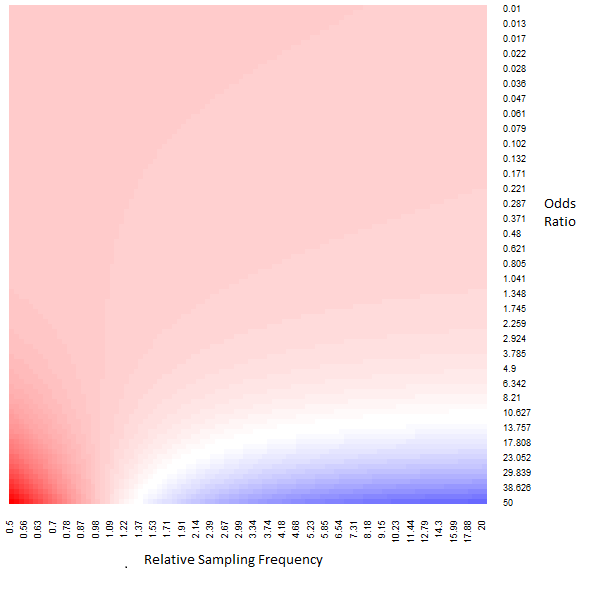
\includegraphics[width = 0.6\textwidth]{../methods/figs/mem_heatmap_article.png}
\caption{Measurement error data quality adjustment: relative frequency $f_1/f_0$ (x-axis) against odds ratio (y-axis) for $FP=0.005$ and $FN=0.172$. Color scaled so blue = $-10$, white = $0$, and red = $10$.}
\label{fig:heatmap}
\end{figure}

% \begin{figure}[!th]
% \centering
% 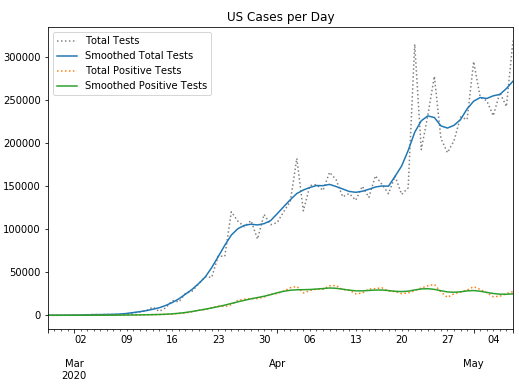
\includegraphics[width = 0.6\textwidth]{../methods/figs/US-casecount.png}
% \caption{US total tests and total positive tests per day}
% \label{fig:ustests}
% \end{figure}

\begin{figure}[!th]
\centering
\begin{subfigure}{.5\textwidth}
  \centering
  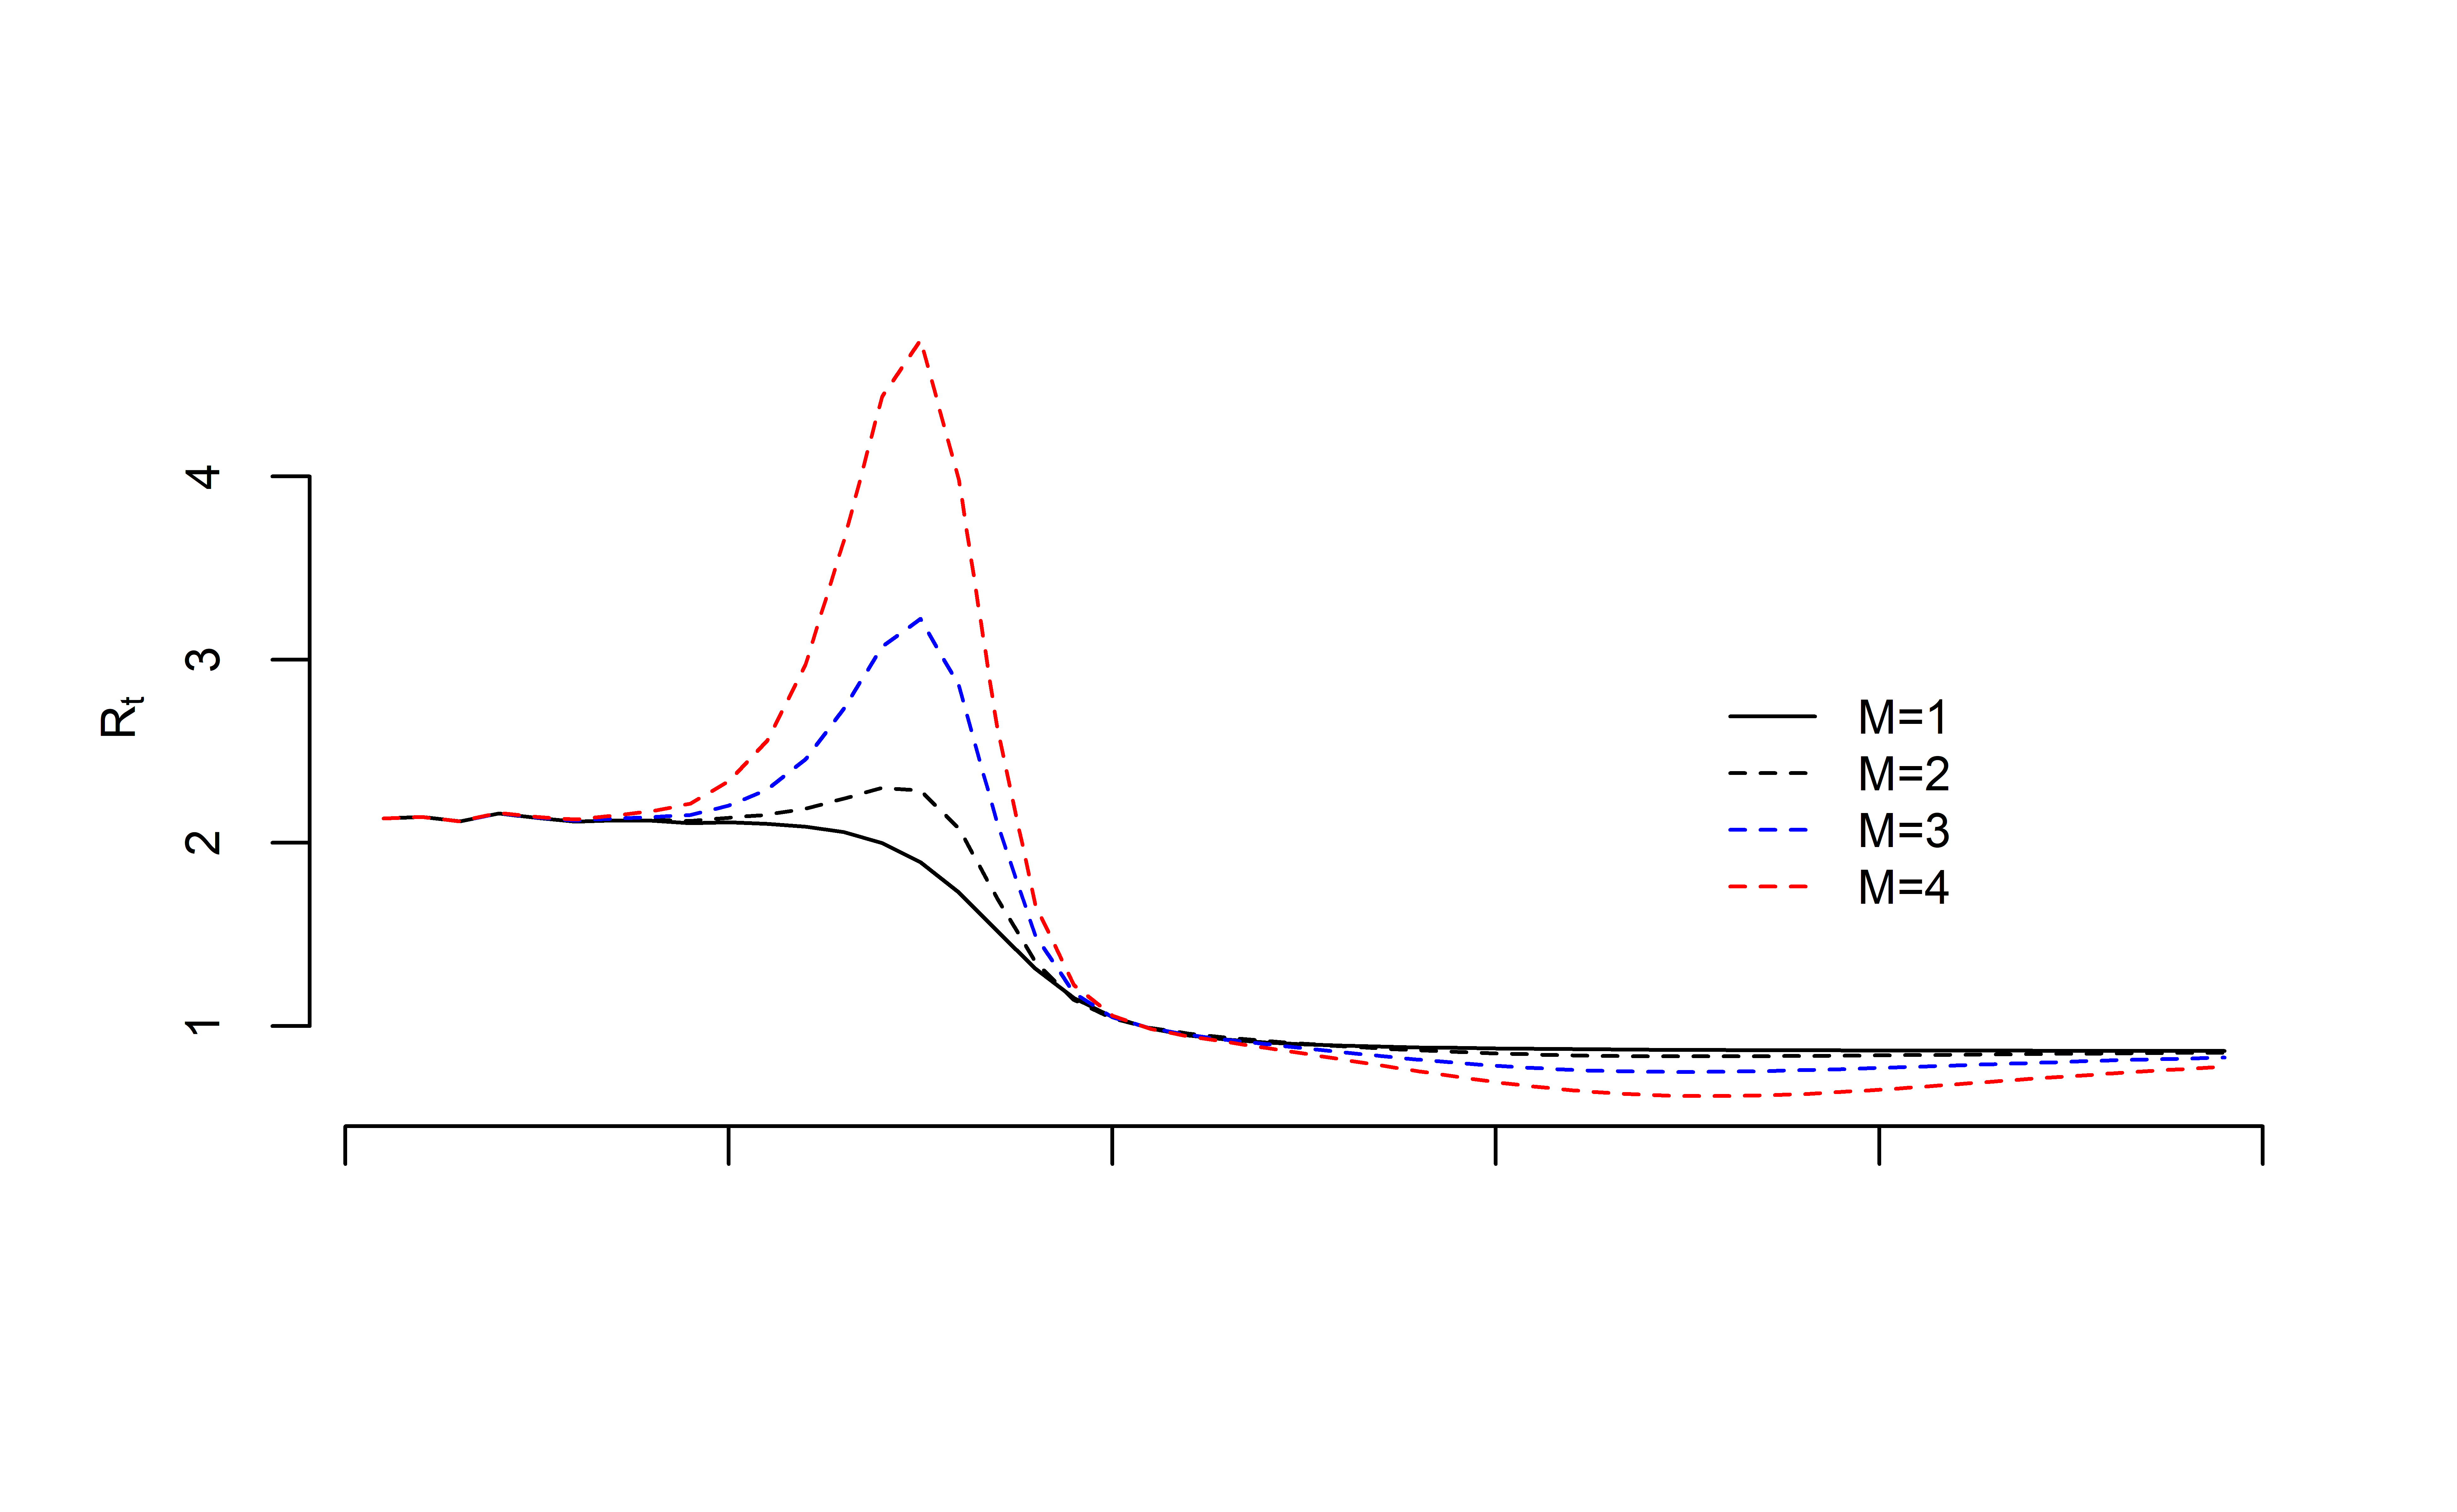
\includegraphics[width=.9\linewidth]{../methods/figs/sir_ratio.png}
  \caption{Ratio estimator}
  \label{fig:ratio-bias}
\end{subfigure}%
\begin{subfigure}{.5\textwidth}
  \centering
  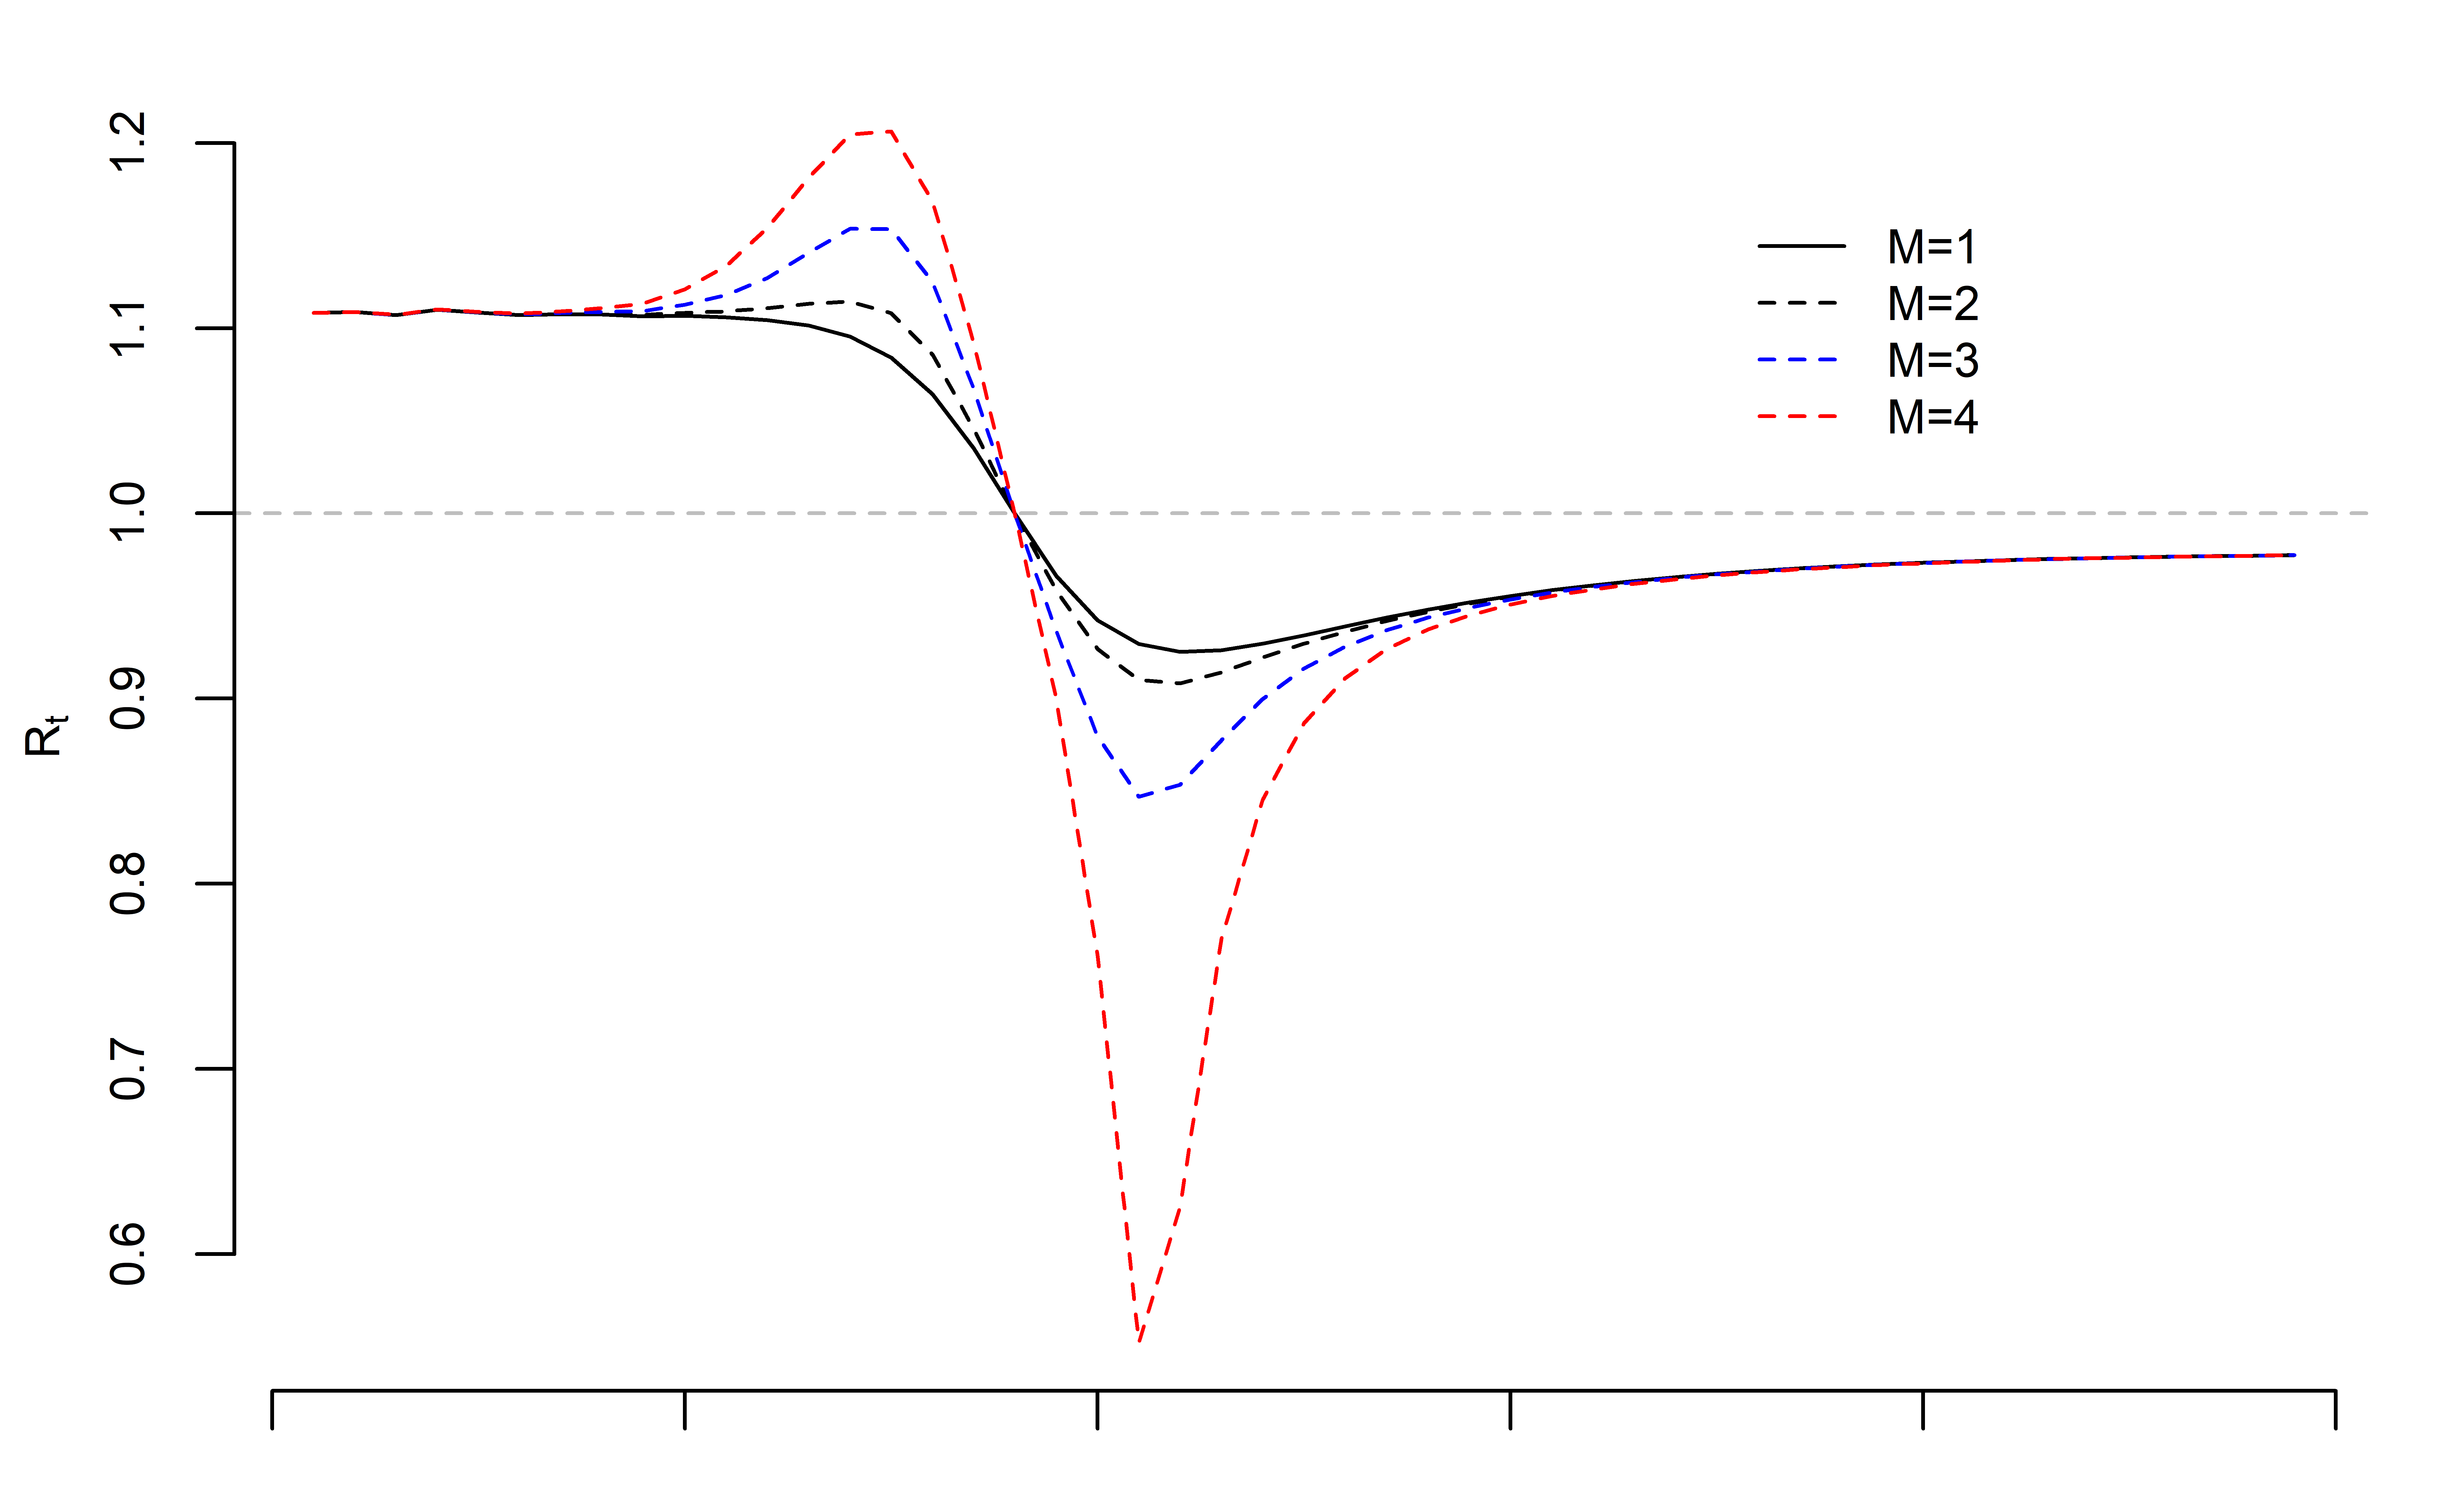
\includegraphics[width=.9\linewidth]{../methods/figs/sir_rt.png}
  \caption{Effective reproductive rate estimator}
  \label{fig:r0-bias}
\end{subfigure}
\caption{Potential bias due to self-selection and measurement error from a deterministic SIR model with $\beta = 1.4$ (black) and $\gamma = 0.2$ (red).  Here we assume $f = 0.02$, $FP = 0.01$, $FN = 0.15$, and use a range of relative sampling fraction $M = f_1/f_0$.}
\label{fig:rates}
\end{figure}

\begin{figure}[!th]
\centering
\begin{subfigure}{.5\textwidth}
  \centering
  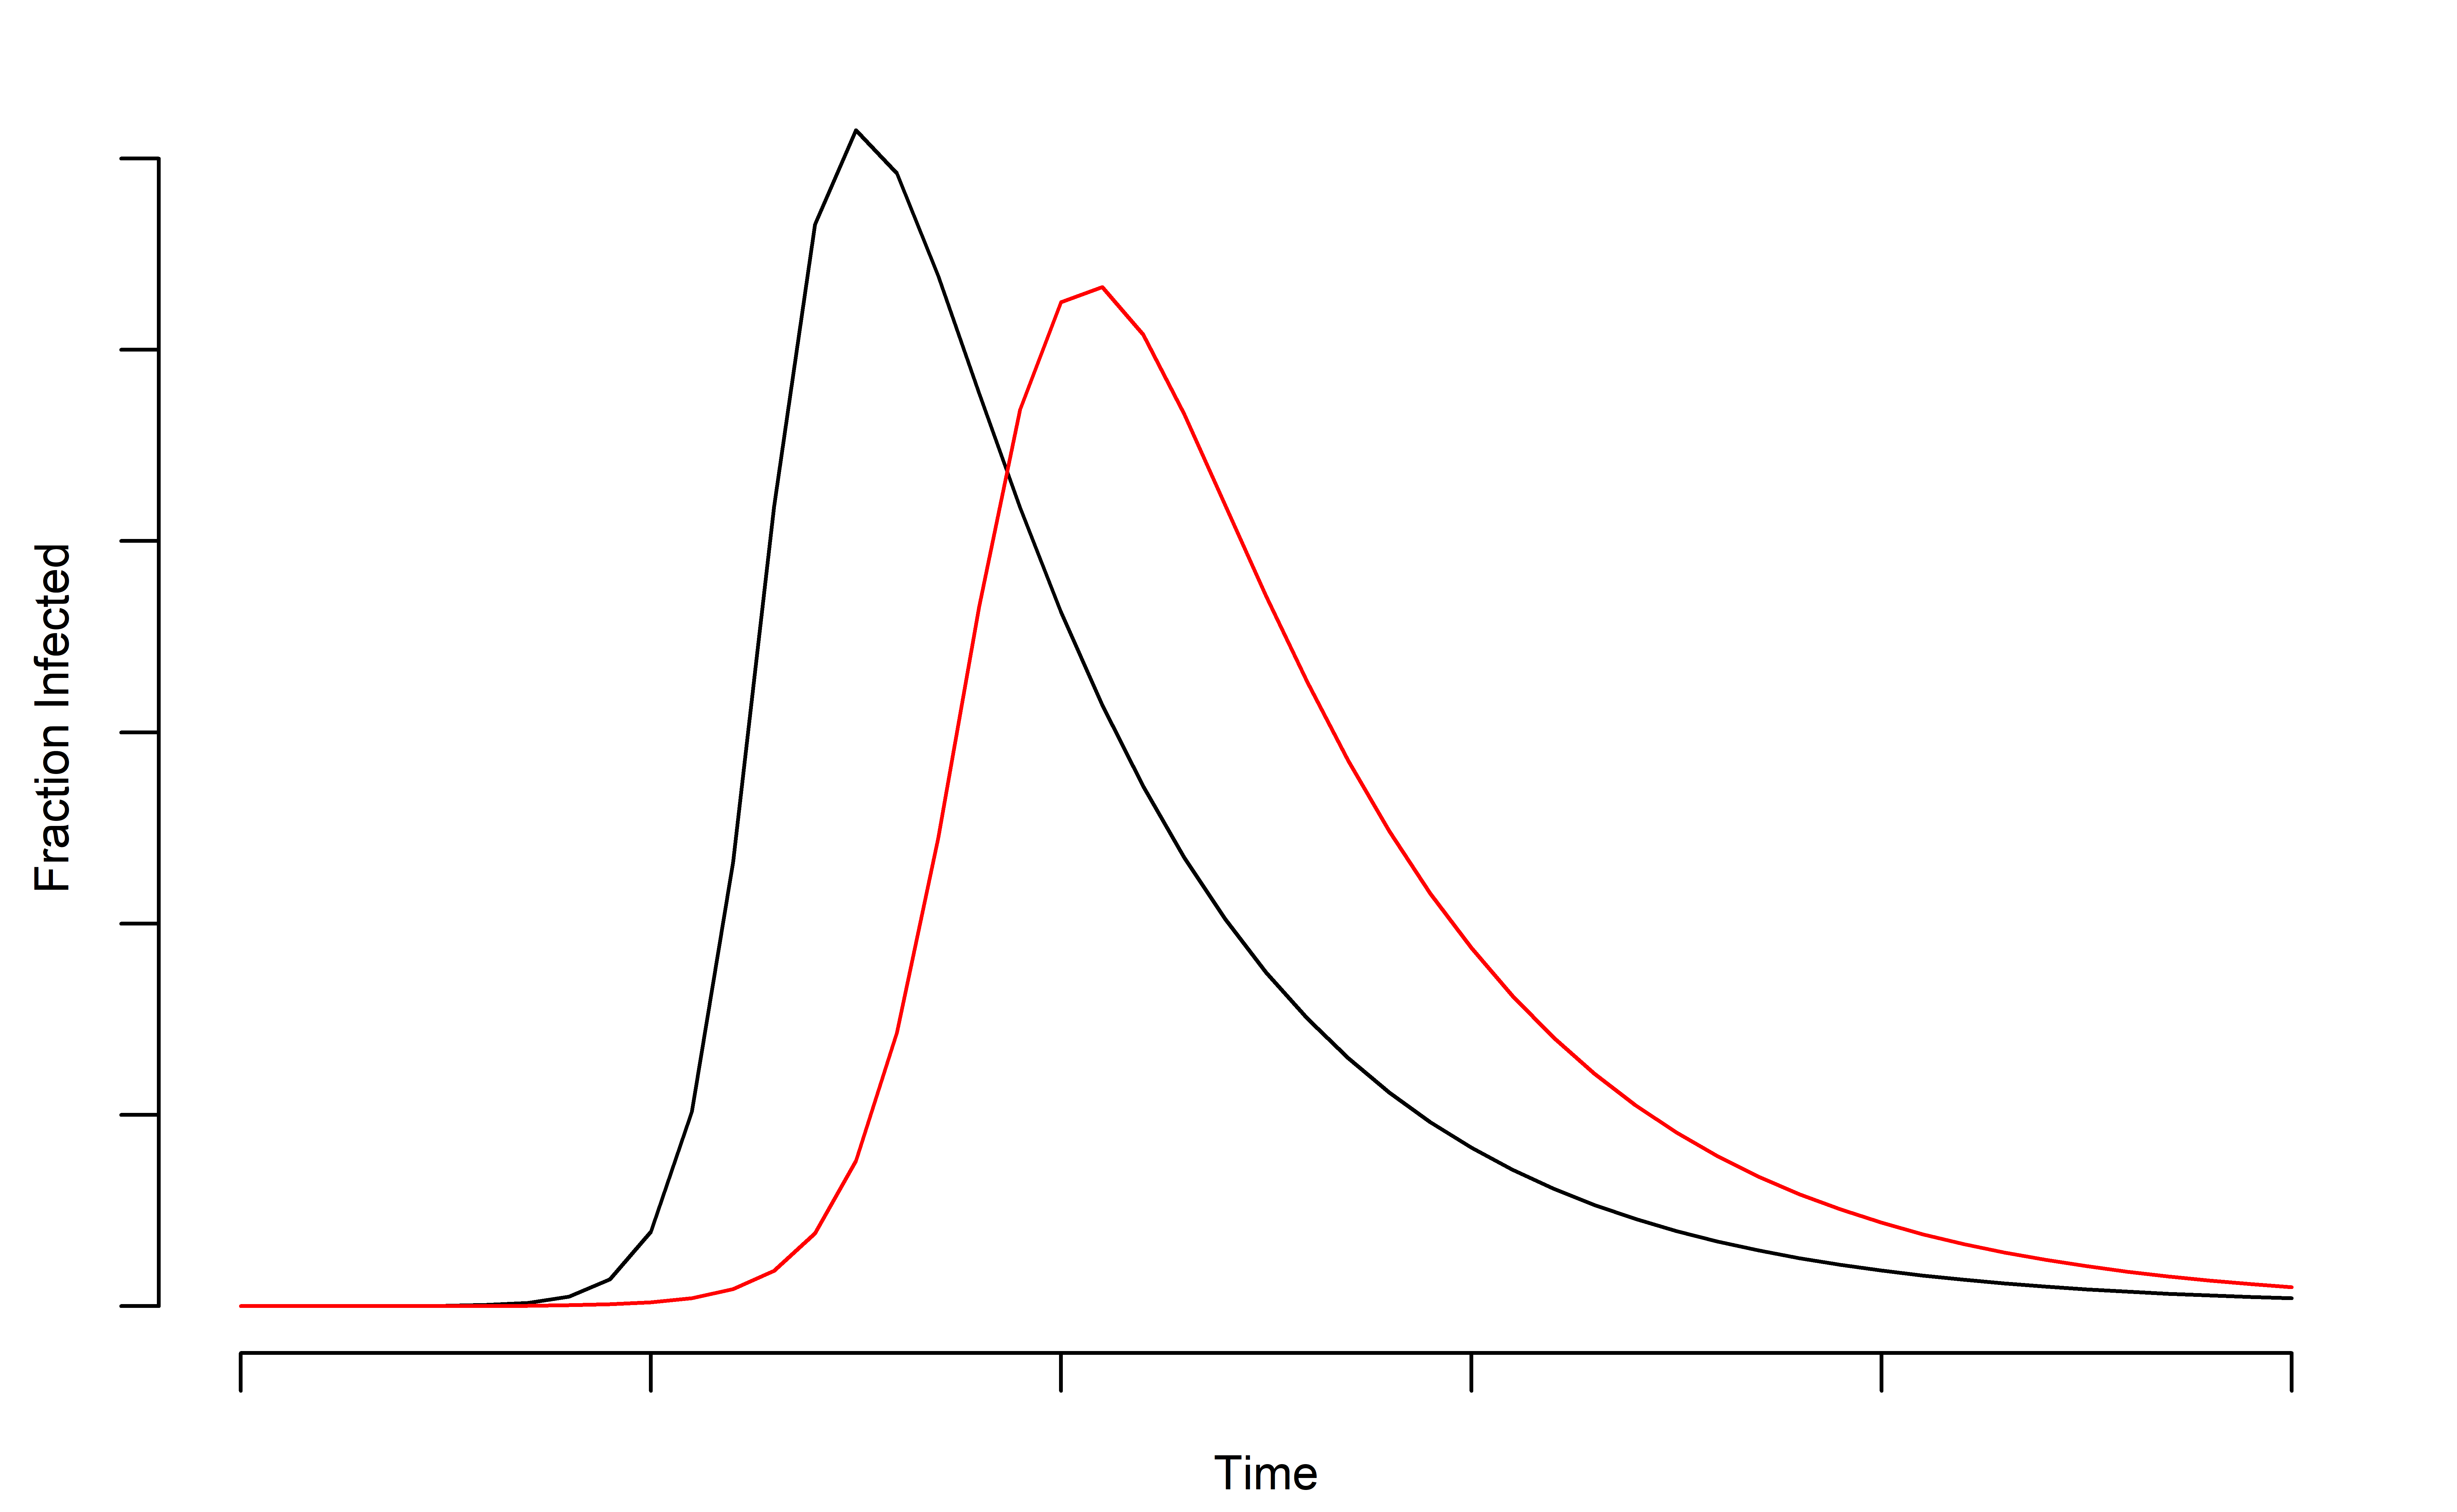
\includegraphics[width=.9\linewidth]{../methods/figs/sir.png}
  \caption{Fraction of new cases in population}
  \label{fig:fracpop}
\end{subfigure}%
\begin{subfigure}{.5\textwidth}
  \centering
  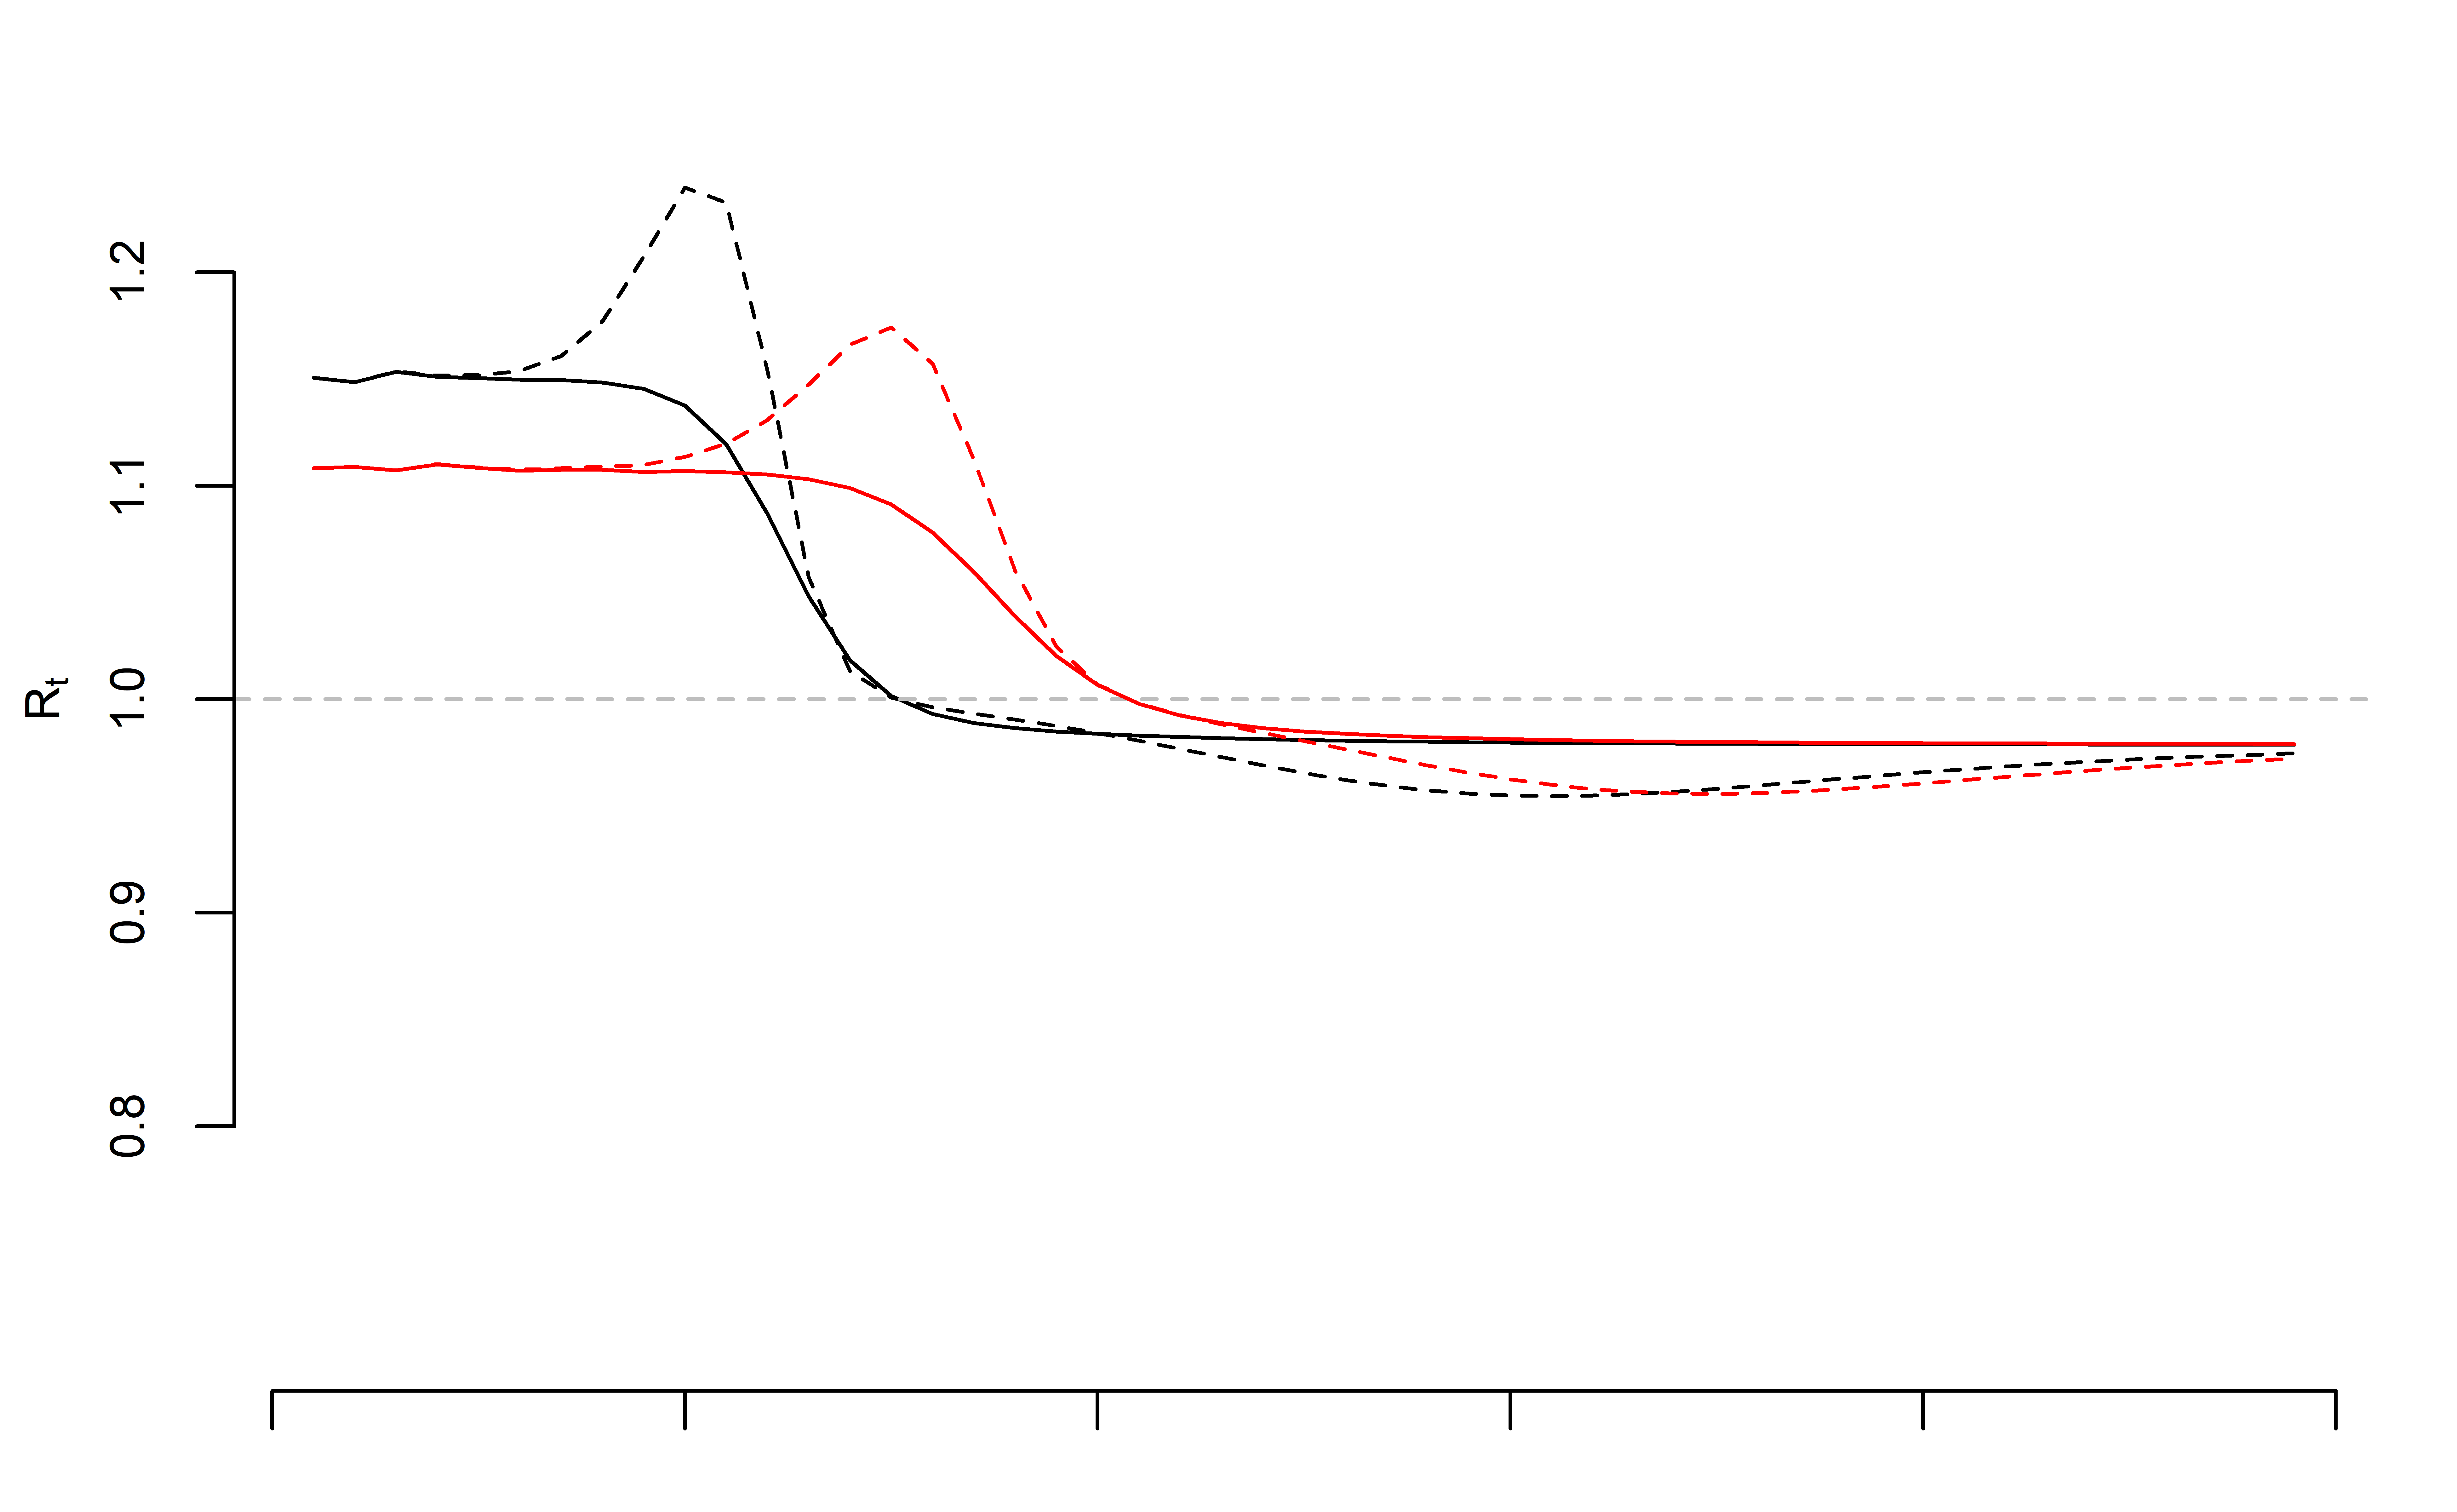
\includegraphics[width=.9\linewidth]{../methods/figs/sir_rt_comparison.png}
  \caption{Effective reproduction rate estimators}
  \label{fig:eff}
\end{subfigure}
\caption{Left: fraction infected in two SIR models with $\beta = 1.4$ and $0.9$ respectively and $\gamma = 0.2$ with same initial conditions. Right: comparison of $\hat R_t$ across time with $FN = 0.2$, $FP = 0.01$, and $M = 4$.}
\label{fig:comparison}
\end{figure}

\begin{figure}[!th]
\centering
\begin{subfigure}{.5\textwidth}
  \centering
  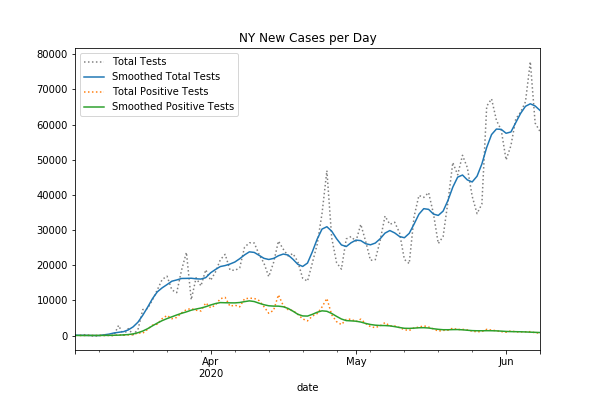
\includegraphics[width=.9\linewidth]{../methods/figs/NY_casecount.png}
  \caption{NY new cases per day}
  \label{fig:ny-covid-test}
\end{subfigure}%
\begin{subfigure}{.5\textwidth}
  \centering
  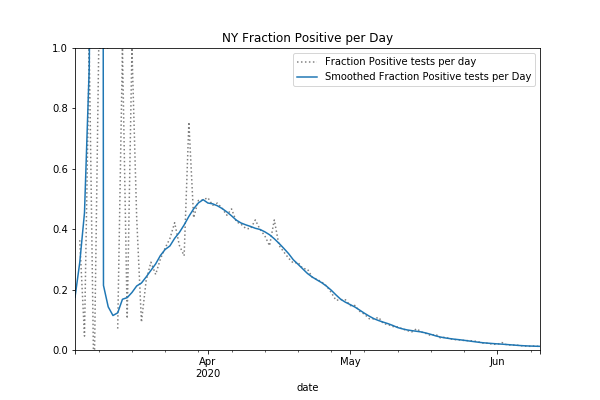
\includegraphics[width=.9\linewidth]{../methods/figs/NY_fracpos.png}
  \caption{NY fraction of new tests positive per day}
  \label{fig:ny-covid-frac}
\end{subfigure}
\caption{New York COVID-19 reported data }
\label{fig:ny-covid}
\end{figure}



% \noindent {\bf Fig. 1.} US total tests and total positive tests per day\\
% \noindent {\bf Fig. 2.} US total tests and total positive tests per day\\
% \noindent {\bf Fig. 3.} US total tests and total positive tests per day\\
% \noindent {\bf Fig. 4.} US total tests and total positive tests per day\\
% \noindent {\bf Fig. 5.} US total tests and total positive tests per day


% Please do not use figure environments to set
% up your figures in the final (post-peer-review) draft, do not include graphics in your
% source code, and do not cite figures in the text using \LaTeX\
% \verb+\ref+ commands.  Instead, simply refer to the figure numbers in
% the text per {\it Science\/} style, and include the list of captions at
% the end of the document, coded as ordinary paragraphs as shown in the
% \texttt{scifile.tex} template file.  Your actual figure files should
% be submitted separately.

\end{document}




















